% Created 2019-02-07 jeu. 15:37
% Intended LaTeX compiler: pdflatex
\documentclass[11pt]{article}
\usepackage[utf8]{inputenc}
\usepackage[T1]{fontenc}
\usepackage{graphicx}
\usepackage{grffile}
\usepackage{longtable}
\usepackage{wrapfig}
\usepackage{rotating}
\usepackage[normalem]{ulem}
\usepackage{amsmath}
\usepackage{textcomp}
\usepackage{amssymb}
\usepackage{capt-of}
\usepackage{hyperref}
\usepackage{minted}
\usepackage[french]{babel}
\usepackage[x11names]{xcolor}
\hypersetup{linktoc = all, colorlinks = true, urlcolor = DodgerBlue4, citecolor = PaleGreen1, linkcolor = black}
\author{Raoul HATTERER}
\date{\today}
\title{Traitement d'image avec commentaires\\\medskip
\large (compléments d'informations à destination du professeur)}
\hypersetup{
 pdfauthor={Raoul HATTERER},
 pdftitle={Traitement d'image avec commentaires},
 pdfkeywords={},
 pdfsubject={},
 pdfcreator={Emacs 26.1 (Org mode 9.2)}, 
 pdflang={French}}
\begin{document}

\maketitle
\tableofcontents

Source : \href{http://www.ac-grenoble.fr/disciplines/informatiquelycee/n\_site/snt\_photo\_transImg.html}{Traitement d'image de l'académie de grenoble}

\section{Installation de PIL}
\label{sec:org729df9a}

À faire au préalable par le professeur.

\begin{minted}[]{shell}
 pip3 install pillow
\end{minted}

\section{La logique RVB}
\label{sec:org5c1f826}

Activité de découverte du RVB: \href{https://www.w3schools.com/colors/colors\_rgb.asp}{colorsRGB}

Pour un pixel, calculer la moyenne des niveaux puis mettre les 3 valeurs à cette moyenne. Essayer pour plusieurs couleurs.

\section{Image de départ}
\label{sec:orgd15b99e}

\begin{figure}[htbp]
\centering
\includegraphics[width=.9\linewidth]{pomme.jpg}
\caption{Image de départ (480px \texttimes{} 300px)}
\end{figure}


\section{Comment lire un pixel}
\label{sec:orgad74a49}

Après avoir fait quelques recherches sur ce qu'est un "pixel", voyons comment lire le pixel de coordonnées (100,250).

\begin{minted}[]{python}
from PIL import Image
img = Image.open("pomme.jpg")
r,v,b=img.getpixel((100,250))
print("canal rouge : ",r,"canal vert : ",v,"canal bleu : ",b)
\end{minted}

\begin{verbatim}
('canal rouge : ', 19, 'canal vert : ', 88, 'canal bleu : ', 192)
\end{verbatim}


\section{Comment écrire un pixel}
\label{sec:org5013023}

\begin{minted}[]{python}
from PIL import Image
img = Image.open("pomme.jpg")
img.putpixel((5,5),(255,0,0))
img.show()
\end{minted}


\section{Que fait le programme suivant ?}
\label{sec:org9d9c5ab}

\begin{minted}[]{python}
from PIL import Image # Importation de la librairie PILLOW (gestion image)
img = Image.open("pomme.jpg") # Mise en mémoire dans la variable "img" le fichier pomme.jpg qui doit être dans le même répertoire que le programme
largeur_image,hauteur_image=img.size # Méthode size aplliquée à la variable img qui renvoie la largeur et la hauteur de l'image
for y in range(hauteur_image): # Pour chaque ligne de 0 à hauteur de l'image
    for x in range(largeur_image): #Pour chaque colonne de 0 à la largeur de chaque ligne
        rouge,vert,bleu=img.getpixel((x,y)) #Méthode getpixels appliquée à la variable img à la position x,y qui renvoie les valeurs r,g,b du pixel.
        nouveau_rouge=vert #le vert devient rouge
        nouveau_vert=bleu #le bleu devient vert
        nouveau_bleu=rouge #le rouge devient bleu
        img.putpixel((x,y),(nouveau_rouge,nouveau_vert,nouveau_bleu)) #Méthode putpixels appliquée à la variable img à la position x,y qui remplace les valeurs r,g,b du pixel.
img.show() #affichage de l'image
img.save("pommeMystere.jpg") #sauvegarde de l'image obtenue
\end{minted}


On analyse le code ci-dessus qui servira de base pour le défi suivant.

\begin{figure}[htbp]
\centering
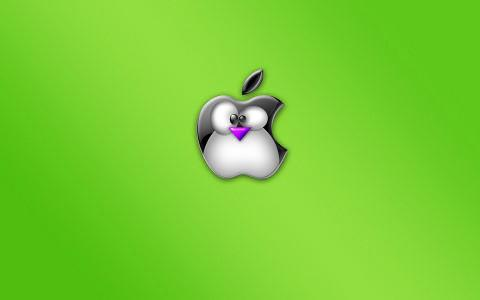
\includegraphics[width=.9\linewidth]{pommeMystere.jpg}
\caption{Résultat du programme mystère}
\end{figure}


\section{Passage d'une image en niveau de gris}
\label{sec:org45bf4bd}

Après avoir fait quelques recherches sur les "images en niveau de gris", écrivez un programme qui transforme une "image couleur" en une "image en niveau de gris".

Petite astuce qui pourrait vous aider : en Python pour avoir une division entière (le résultat est un entier), il faut utiliser l'opérateur // à la place de l'opérateur / 

Remarque: On donne l'algorithme aux élèves (ou on le construit avec eux) ; ils doivent alors programmer le passage d'une image couleur à une image en niveaux de gris.


\begin{minted}[]{python}
from PIL import Image
img = Image.open("pomme.jpg")
largeur_image=480
hauteur_image=300
for y in range(hauteur_image):
    for x in range(largeur_image):
       rouge,vert,bleu=img.getpixel((x,y))
       nouveau_rouge=(vert+bleu+rouge)//3
       nouveau_vert=(vert+bleu+rouge)//3
       nouveau_bleu=(vert+bleu+rouge)//3
       img.putpixel((x,y),(nouveau_rouge,nouveau_vert,nouveau_bleu))
img.show()
img.save("pommegrise.jpg")
\end{minted}

\begin{figure}[htbp]
\centering
\includegraphics[width=.9\linewidth]{pommegrise.jpg}
\caption{Image en niveaux de gris}
\end{figure}
\end{document}